\documentclass[a4paper,10pt]{article}

% рисунки
\usepackage{graphicx}

\usepackage[T2A]{fontenc}
\usepackage[utf8]{inputenc}
\usepackage[english,russian]{babel}

\RequirePackage{caption}
\DeclareCaptionLabelSeparator{defffis}{ — }
\captionsetup{justification=centering,labelsep=defffis}

\usepackage{caption} \captionsetup[table]{labelsep=endash,justification=justified,singlelinecheck=false,font=normalsize}

\usepackage{amsmath,amsfonts,amssymb,amsthm,mathtools}



\begin{document}
  
\begin{center}
  \section*{Лабораторная работа №3.3.4 \\Эффект Холла в полупроводниках\\Джокер Бэтмен, Б02-000, 25.09.2021}
\end{center}  

\vspace{5mm}
\section*{Введение}

\begin{flushleft}
  \textbf{Цель работы:} измерение подвижности и концентрации носителей заряда в полупроводниках.

\end{flushleft}

\begin{flushleft}
  \textbf{В работе используются:} электромагнит с источником иптания GPR, батарейка 1,5 В, амперметр, реостат, цифровой вольтмет В7-78/1, милливеберметр, образцы легированного германия.

\end{flushleft}

\section*{Теоретическая справка}

\subsection*{Эффект Холла}

Во внешнем магнитном поле $\vec{B}$ на заряды действует сила Лоренца:\[\vec{F}=q\vec{E}+q\vec{u}\times\vec{B}.\]Эта сила вызывает движение носителей, направление которого в общем случае не совпадает с $\vec{E}$. Действительно, траектории частиц будут либо искривляться, либо, если геометрия проводника этого не позволяет, возникнет дополнительное электрическое поле, компенсирующее магнитную составляющую силы Лорнеца. Возникновение попречного току электрического поля в образце, помещённом во внешнее магнитное поле, называют \textit{эффектом Холла}.

\subsection*{Мостик Холла}

\begin{figure}[h]
	\centering
	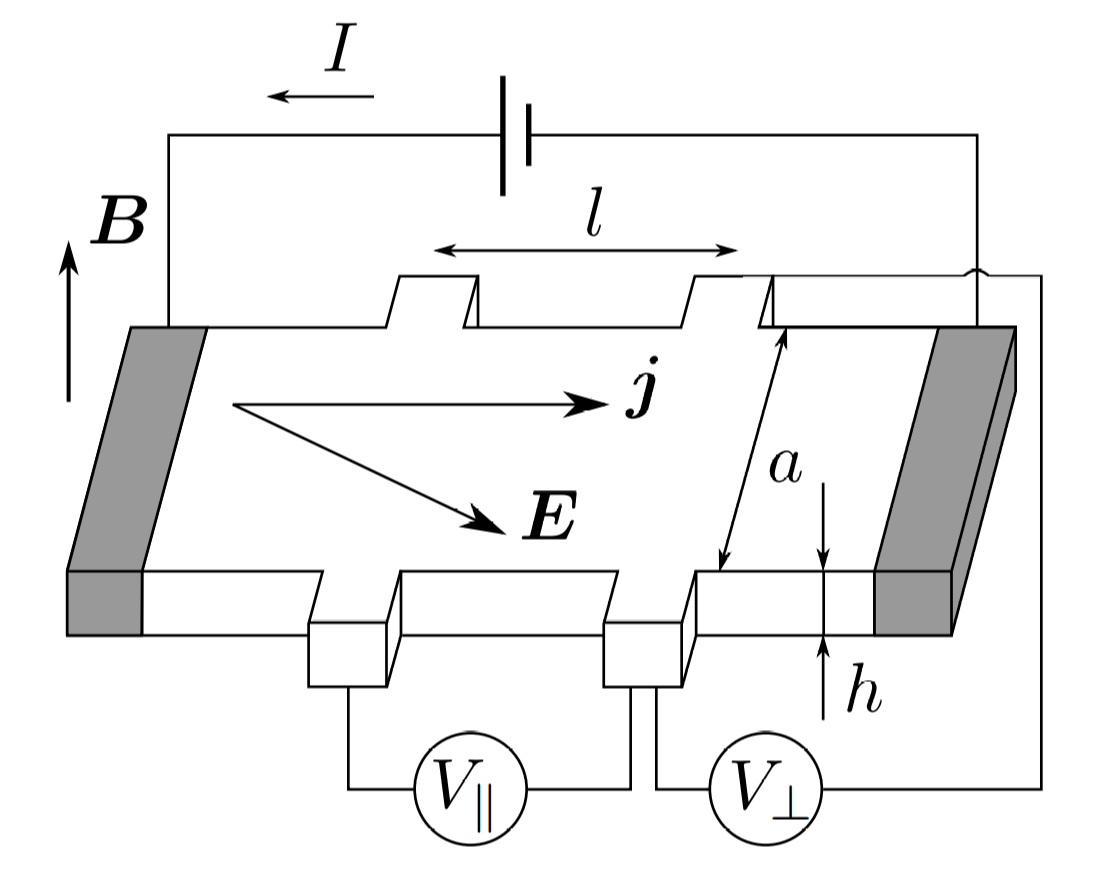
\includegraphics[scale=0.35]{th}
	\caption{Схема мостика Холла} \label{th}
\end{figure}

Для исследования завиисимости проводимости среды от магнитного поля используют т.н. \textit{мостик Холла}. В данной схеме (см. рисунок \Ref{th}) ток вынуждают течь по оси $x$ вдоль плоской пластинки (ширина пластинки $a$, толщина $h$, длина $l$). Сила Лоренца, действующая со стороны перпендикулярного пластинке магнитного поля, "прибивает" носители заряда к краям образца, что создаёт холловское электрическое поле, компенсирующее эту силу. Поперечное напряжение между краями пластинки (\textit{холловское напряжение}) равно $U_{\perp}=E_ya$, где\[E_y=\frac{j_xB}{nq}.\]Плотность тока, текущего через образец, равна $j_x=\frac{I}{ah}$, где $I$ -- полный ток, $ah$ -- поперечное сечение. Таким образом, для холловского напряжения имеем\[U_{\perp}=\frac{B}{nqh}I=R_H\frac{B}{h}I,\]где константу\[R_H=\frac{1}{nq}\]называют \textit{постоянной Холла}. Знак постоянной Холла определяется знаком заряда носителей.

Продольная напряжённость электрического поля равна\[E_x=\frac{j_x}{\sigma_0},\]и падение напряжения $U_{\parallel}=E_xl$ \textit{вдоль} пластинки определяется омическим сопротивлением образца $R_0=\frac{l}{\sigma_0ah}$:\[U_{\parallel}=IR_0.\]Интересно отметить, что немотря на то, что тензор проводимости явно зависит от $B$, продольное сопротивление образца в данной геометрии от магнитного поля \textit{не зависит}.

\section*{Экспериментальная установка}

Электрическая схема установки для измерения ЭДС Холла представлена на рисунке \Ref{Device}. 

\begin{figure}[h]
	\centering
	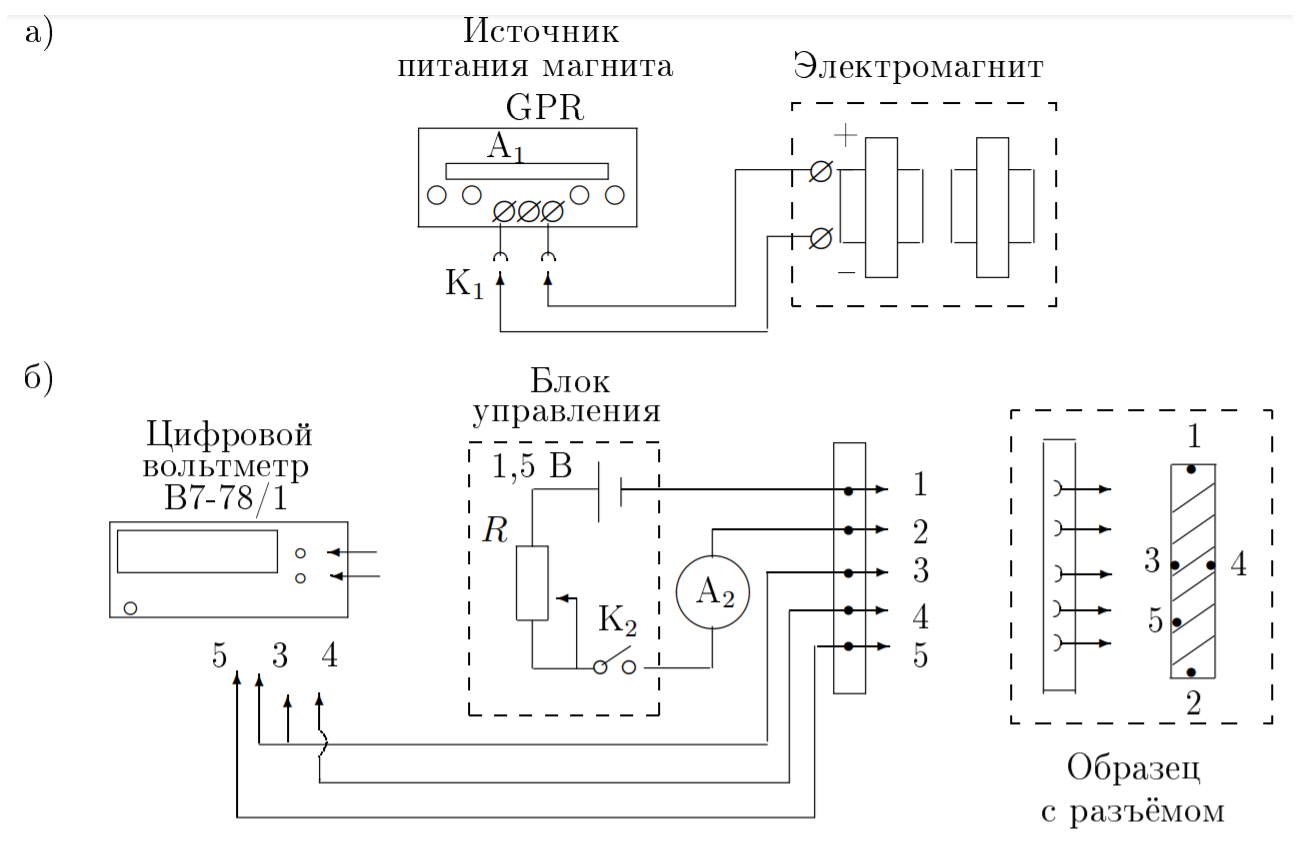
\includegraphics[scale=0.35]{Device}
	\caption{Схема установки для исследования эффекта Холла в полупроводниках} \label{Device}
\end{figure}

В зазоре электромагнита создаётся постоянное магнитное поле, величину которого можно менять с помощью регуляторов источника питания. Ток измеряется амперметров источника питания $A_1$. Разъём $K_1$ позволяет менять направление тока в обмотках электромагнита.

Градуировка магнита проводится при помощи милливеберметра.

Образец из легированного германия, смонтированный в специальном держателе, подключается к батарее ($\approx1,5~\text{В}$). При замыкании ключа $K_2$ вдоль длинной стороны образца течёт ток, величина которого регулируется реостатом $R$ и измеряется миллиамперметром $A_2$.

В образце с током, помещённом в зазор электромагнита, между контактами 3 и 4 возникает разность потенциалов $U_{34}$, которая измеряется с помощью цифрового вольтметра.

Контакты 3 и 4 вследствие неточности подпайки не всегда лежат на одной эквипотенциали, и тогда напряжение между ними связано не только с эффектом Холла, но и с омическим падением напряжения, вызванным протеканием основного тока через образец. Измеряемая разность потенциалов при одном направлении магнитного поля равна сумме ЭДС Холла и омического падения напряжения, а при другом -- их разности. В этом случае ЭДС Холла $\varepsilon_{\text{Х}}$ может быть определена как половина алгебраической разности показаний вольтметра, полученных для двух противоположных направлений магнитного поля в зазоре. Знак измеряемого напряжения высвечивается на цифровом табло вольтметра.

Можно исключить влияние омического падения напряжения иначе, если при каждом токе через образец измерять напряжение между точками 3 и 4 в отсутствие магнитного поля. При фиксированном токе через образец это дополнительное к ЭДС Холла напряжение $U_0$ остаётся неизменным. От него следует (с учётом знака) отсчитывать величину ЭДС Холла: $\varepsilon_{\text{Х}}=U_{34}\pm U_0$. При таком способе измерения нет неообходимости проводить повторные измерения с противоположным направлением магнитного поля.

По знаку $\varepsilon_{\text{Х}}$ можно определить характер проводимости -- электронный или дырочный. Для этого необходимо знать направление тока в образце и направление магнитного поля. Измерив ток $I$ в образце и напряжение $U_{35}$ между контактами 3 и 5 в отсутствие магнитного поля, можно, зная параметры образца, рассчитать проводимость материала образца по очевидной формуле:\[\sigma=\frac{IL_{35}}{U_{35}al},\]где $L_{35}$ -- расстояние между контактами 3 и 5, $a$ -- толщина образца, $l$ -- его ширина.

\section*{Ход работы}

Параметры образца германия, используемого в работе: толщина $a=2,2~\text{мм}$, ширина $l=7~\text{мм}$, расстояние между контактами 3 и 5 $L_{35}=6,0~\text{мм}$.

\subsection{I. Градуировка электромагнита}

С помощью милливеберметра снимем зависимость магниного потока $\Phi$, пронизывающего пробную катушку, находящуюся в зазоре, от тока $I_M$ ($\Phi=BSN$, где значение $SN=72~\text{см}^2=7,2\cdot10^{-3}~\text{м}^2$ -- произведение площади сечения пробной катушки на число витков в ней -- указано на установке (погрешностью его пренебрежём)). Для измерения магнитного потока необходимо сначала поместить пробную катушку в зазор электромагнита и записать показания милливеберметра $\Phi_1$ при этом. Затем её нужно очень быстро убрать из зазора и записать показания милливеберметра $\Phi_2$. Разность $\Phi_1-\Phi_2$ и будет определять величину магнитного потока $\Phi$ через пробную катушку, откуда с лёгкостью можно найти соответствующую величину магнитного поля $B$. Проведём измерения при 8 различных значениях тока $I_M$ вдполь до макисмального $I_{Mmax}=1,65~\text{А}$. Все полученные данные занесём в таблицу \Ref{kal}. В дальнейшем будем учитывать также погрешность милливеберметра. При измерении $\Phi=\Phi_1-\Phi_2$ погрешность равна $\sigma_{\Phi}=\sqrt{\sigma_{\Phi_1}^2+\sigma_{\Phi_2}^2}=\sqrt2\Delta\Phi$, откуда погрешность определения индукции магнитного поля равна $\sigma_B=\frac{\sigma_{\Phi}}{SN}=\frac{\sqrt2\Delta\Phi}{SN}\approx0,01~\text{Тл}$. Погрешность измерения тока будет равна $\sigma_I=0,005I+0,02~\text{А}$, также внесём её в таблицу.

\begin{table}[h]
	\centering
	\caption{Зависимость индукции магнитного поля $B$ в зазоре электромагнита от тока $I_M$ через обмотки} \label{kal}
	\begin{tabular}{|c|c|c|c|c|c|c|c|c|}
		\hline
		$I_M$, А & 0,20 & 0,41 & 0,61 & 0,82 & 1,03 & 1,24 & 1,44 & 1,65 \\ \hline
		$\sigma_I$, А & 0,02 & 0,02 & 0,02 & 0,02 & 0,03 & 0,03 & 0,03 & 0,03 \\ \hline
		$\Phi_1$, мВб & 5,1 & 6,2 & 7,1 & 7,0 & 7,9 & 7,7 & 8,1 & 8,4 \\ \hline
		$\Phi_2$, мВб & 3,9 & 3,9 & 3,8 & 2,6 & 2,6 & 1,8 & 1,7 & 1,7 \\ \hline
		$\Phi$, мВб & 1,2 & 2,3 & 3,3 & 4,4 & 5,3 & 5,9 & 6,4 & 6,7 \\ \hline
		$B$, Тл & 0,17 & 0,32 & 0,46 & 0,61 & 0,74 & 0,82 & 0,89 & 0,93 \\ \hline
	\end{tabular}
\end{table}

Пользуясь значениями из таблицы \Ref{kal}, построим теперь градуировочную кривую для электромагнита $B(I_M)$. Результат приведён ниже на графике \Ref{kkal}.

\begin{figure}[h]
	\centering
	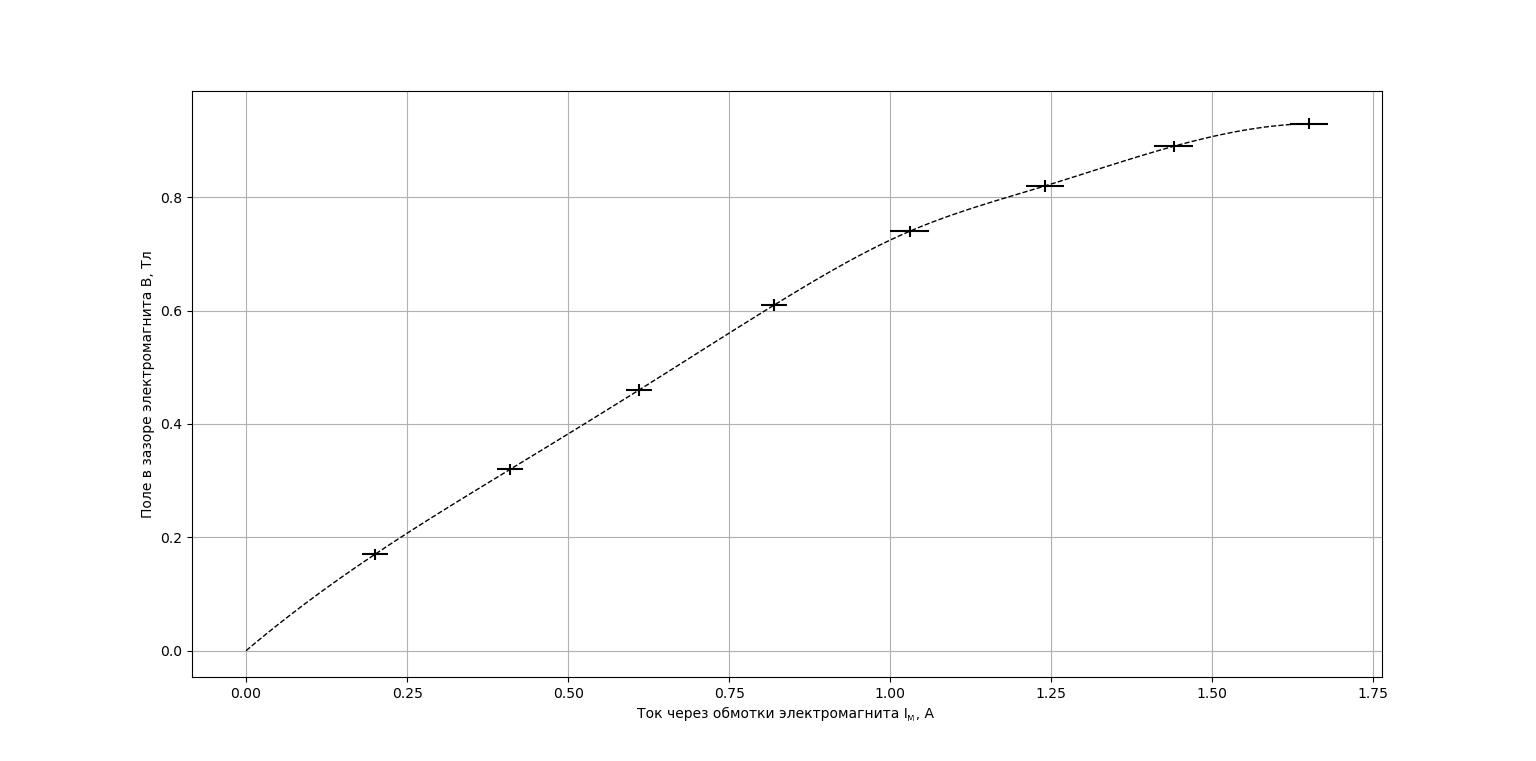
\includegraphics[scale = 0.33]{kkal}
	\caption{Градуировочная кривая $B(I_M)$ для электромагнита. Сглаживающая кривая проведена с помощью кубических сплайнов} \label{kkal}
\end{figure} 

\subsection*{II. Измерение ЭДС Холла}

Вставим держатель с образцом в зазор электромагнита. Установим по миллиамперметру минимальное значение тока через образец (в нашем случае $I_{min}-0,14~\text{мА}$). В отсутствие магнитного поля вольтметр будет показывать постоянное напряжение $U_0$, вызванное несовершенством контактов 3, 4 и наводками. Будем в дальнейшем учитывать это значение и для каждого значения тока через образец принимать $U_0$ за начало отсчёта. Проведём измерения $U_{34}(I_M)$ для нескольких значений тока в диапазоне от $I_{min}$ до $I_{max}=1,00~\text{мА}$. При максимальном токе также проведём измерения при другом направлении магнитного поля через образец. Вычислим по этим данным ЭДС Холла $\varepsilon_{\text{Х}}$. Все результаты занесём в таблицы \Ref{hol} и \Ref{holl}.

\begin{table}[h]
	\centering
	\caption{Зависимость $U_0$ от $I$} \label{hol}
	\begin{tabular}{|c|c|c|c|c|c|c|c|c|c|c|}
		\hline
		$I$,А&0,14&0,25&0,35&0,44&0,53&0,63&0,72&0,81&0,91&1,00\\ \hline
		$U_0$,мкВ&-19&-36&-50&-64&-77&-92&-106&-119&-134&-148\\ \hline
	\end{tabular}
\end{table}

\begin{table}
	\centering
	\caption{Зависимость $U_{34}$ от $I_M$ при токах через образец, указанных в таблице \Ref{hol}} \label{holl}
	\begin{tabular}{|c|c|c|c|c|c|c|c|c|}
		\hline
		$I_M$, А & 0,20 & 0,41 & 0,61 & 0,82 & 1,03 & 1,24 & 1,44 & 1,60 \\ \hline
		$U_{34}$, мкВ & -8 & 1 & 11 & 19 & 26 & 30 & 33 & 35 \\ \hline
		$B$, Тл & 0,17 & 0,32 & 0,46 & 0,61 & 0,74 & 0,82 & 0,89 & 0,93 \\ \hline
		$\varepsilon_{\text{Х}}$, мкВ & 11 & 20 & 30 & 38 & 45 & 49 & 52 & 54 \\ \hline
		\hline
		$I_M$, А & 0,20 & 0,41 & 0,61 & 0,82 & 1,03 & 1,24 & 1,44 & 1,59 \\ \hline
		$U_{34}$, мкВ & -16 & 3 & 20 & 35 & 47 & 55 & 60 & 63 \\ \hline
		$B$, Тл & 0,17 & 0,32 & 0,46 & 0,61 & 0,74 & 0,82 & 0,89 & 0,93 \\ \hline
		$\varepsilon_{\text{Х}}$, мкВ & 20 & 39 & 56 & 71 & 83 & 91 & 96 & 99 \\ \hline
		\hline
		$I_M$, А & 0,20 & 0,41 & 0,61 & 0,82 & 1,03 & 1,24 & 1,44 & 1,59 \\ \hline
		$U_{34}$, мкВ & -23 & 4 & 27 & 50 & 67 & 77 & 85 & 89 \\ \hline
		$B$, Тл & 0,17 & 0,32 & 0,46 & 0,61 & 0,74 & 0,82 & 0,89 & 0,93 \\ \hline
		$\varepsilon_{\text{Х}}$, мкВ & 27 & 54 & 77 & 100 & 117 & 127 & 135 & 139 \\ \hline
		\hline
		$I_M$, А & 0,20 & 0,41 & 0,61 & 0,82 & 1,03 & 1,24 & 1,44 & 1,58 \\ \hline
		$U_{34}$, мкВ & -30 & 5 & 34 & 61 & 83 & 98 & 107 & 111 \\ \hline
		$B$, Тл & 0,17 & 0,32 & 0,46 & 0,61 & 0,74 & 0,82 & 0,89 & 0,92 \\ \hline
		$\varepsilon_{\text{Х}}$, мкВ & 34 & 69 & 98 & 125 & 147 & 162 & 171 & 175 \\ \hline
		\hline
		$I_M$, А & 0,20 & 0,41 & 0,61 & 0,82 & 1,03 & 1,24 & 1,44 & 1,58 \\ \hline
		$U_{34}$, мкВ & -36 & 6 & 41 & 75 & 100 & 118 & 128 & 134 \\ \hline
		$B$, Тл & 0,17 & 0,32 & 0,46 & 0,61 & 0,74 & 0,82 & 0,89 & 0,92 \\ \hline
		$\varepsilon_{\text{Х}}$, мкВ & 41 & 83 & 118 & 152 & 177 & 195 & 205 & 211 \\ \hline
		\hline
		$I_M$, А & 0,20 & 0,41 & 0,61 & 0,82 & 1,03 & 1,24 & 1,44 & 1,57 \\ \hline
		$U_{34}$, мкВ & -43 & 7 & 48 & 88 & 119 & 140 & 153 & 159 \\ \hline
		$B$, Тл & 0,17 & 0,32 & 0,46 & 0,61 & 0,74 & 0,82 & 0,89 & 0,92 \\ \hline
		$\varepsilon_{\text{Х}}$, мкВ & 49 & 99 & 140 & 180 & 211 & 232 & 245 & 251 \\ \hline
		\hline
		$I_M$, А & 0,20 & 0,41 & 0,61 & 0,82 & 1,03 & 1,24 & 1,44 & 1,57 \\ \hline
		$U_{34}$, мкВ & -49 & 7 & 55 & 103 & 135 & 160 & 174 & 181 \\ \hline
		$B$, Тл & 0,17 & 0,32 & 0,46 & 0,61 & 0,74 & 0,82 & 0,89 & 0,92 \\ \hline
		$\varepsilon_{\text{Х}}$, мкВ & 57 & 113 & 161 & 209 & 241 & 266 & 280 & 287 \\ \hline
		\hline
		$I_M$, А & 0,20 & 0,41 & 0,61 & 0,82 & 1,03 & 1,24 & 1,44 & 1,55 \\ \hline
		$U_{34}$, мкВ & -57 & 7 & 62 & 115 & 154 & 178 & 196 & 202 \\ \hline
		$B$, Тл & 0,17 & 0,32 & 0,46 & 0,61 & 0,74 & 0,82 & 0,89 & 0,92 \\ \hline
		$\varepsilon_{\text{Х}}$, мкВ & 62 & 126 & 181 & 234 & 273 & 297 & 315 & 321 \\ \hline
		\hline
		$I_M$, А & 0,20 & 0,41 & 0,61 & 0,82 & 1,03 & 1,24 & 1,44 & 1,55 \\ \hline
		$U_{34}$, мкВ & -63 & 8 & 69 & 128 & 171 & 198 & 220 & 228 \\ \hline
		$B$, Тл & 0,17 & 0,32 & 0,46 & 0,61 & 0,74 & 0,82 & 0,89 & 0,92 \\ \hline
		$\varepsilon_{\text{Х}}$, мкВ & 71 & 142 & 203 & 262 & 305 & 332 & 354 & 362 \\ \hline
		\hline
		$I_M$, А & 0,20 & 0,41 & 0,61 & 0,82 & 1,03 & 1,24 & 1,44 & 1,55 \\ \hline
		$U_{34}$, мкВ & -72 & 8 & 76 & 140 & 188 & 219 & 241 & 250 \\ \hline
		$B$, Тл & 0,17 & 0,32 & 0,46 & 0,61 & 0,74 & 0,82 & 0,89 & 0,92 \\ \hline
		$\varepsilon_{\text{Х}}$, мкВ & 76 & 156 & 224 & 288 & 336 & 367 & 389 & 398 \\ \hline
		\hline
		$I_M$, А & -0,20 & -0,41 & -0,61 & -0,82 & -1,03 & -1,24 & -1,44 & -1,55 \\ \hline
		$U_{34}$, мкВ & -238 & -322 & -393 & -465 & -518 & -551 & -572 & -582 \\ \hline
		$B$, Тл & 0,17 & 0,32 & 0,46 & 0,61 & 0,74 & 0,82 & 0,89 & 0,92 \\ \hline
		$\varepsilon_{\text{Х}}$, мкВ & -75 & -159 & -230 & -302 & -355 & -388 & -409 & -419 \\ \hline
	\end{tabular}
\end{table}

По данным из таблицы \Ref{holl} построим семейство характеристик $\varepsilon_{\text{Х}}(B)$ при разных значениях тока через образец (показано ниже на рисунке \Ref{hui}). Для измерений с обратной полярностью на максимальном токе построим модуль ЭДС Холла. Определим с помощью МНК угловые коэффициенты $K(I)\equiv\frac{\Delta\varepsilon}{\Delta B}$ полученных прямых. Для максимального тока возьмём среднее значение угловых коэффициентов. Внесём данные в таблицу \Ref{hhui}.

\begin{figure}[h]
	\centering
	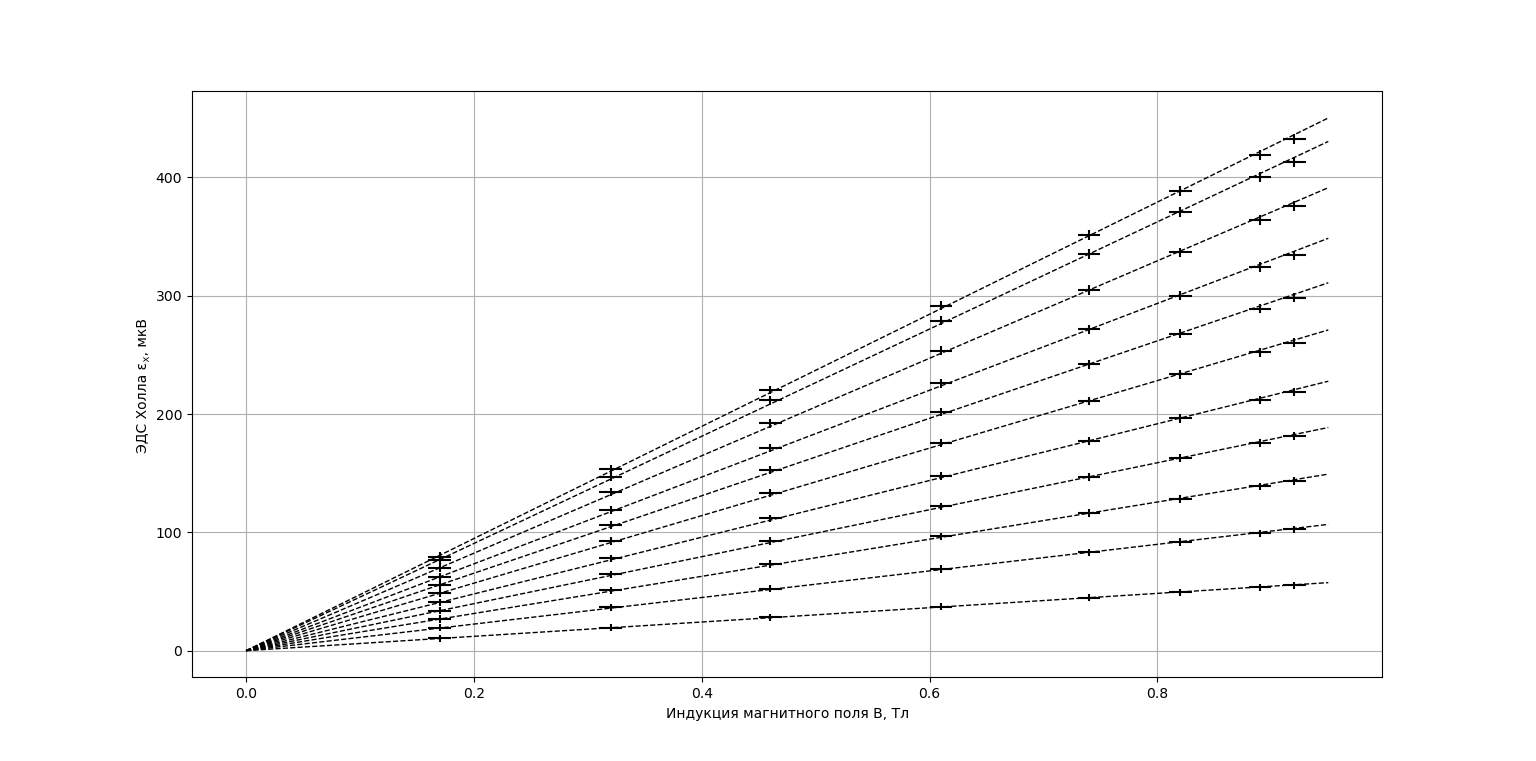
\includegraphics[scale = 0.33]{hui}
	\caption{Семейство характеристик $\varepsilon_{\text{Х}}(B)$ при различных значениях тока через образец. Прямые проведены с помощью МНК} \label{hui}
\end{figure} 

\begin{table}[h]
	\centering
	\caption{Зависимость $K$ от $I$} \label{hhui}
	\begin{tabular}{|c|c|c|c|c|c|c|c|c|c|c|}
		\hline
		$I$,А&0,14&0,25&0,35&0,44&0,53&0,63&0,72&0,81&0,91&1,00\\ \hline
		$K,\frac{\text{мкВ}}{\text{Тл}}$&60,5&112,3&157,1&198,6&239,8&285,4&327,4&366,9&412,0&463,6\\ \hline
		$\sigma_K,\frac{\text{мкВ}}{\text{Тл}}$&3,2&3,4&3,6&3,7&3,9&4,0&4,2&4,3&4,5&4,6\\ \hline
	\end{tabular}
\end{table}

Построим теперь график $K(I)$, он представлен ниже на рисунке \Ref{hhhui}. Угловой коэффициент прямой на графике можно найти с помощью МНК. Он равен $\frac{\Delta K}{\Delta I}=\left(453,9\pm4,7\right)~\frac{\text{мкВ}}{\text{мА}\cdot\text{Тл}}=\left(0,4539\pm0,0047\right)~\frac{\text{В}}{\text{А}\cdot\text{Тл}}$. Тогда постоянную Холла можно найти как\[R_{\text{Х}}=a\frac{\Delta K}{\Delta I}=\left(2,66\pm0,04\right)\cdot10^{-1}~\frac{\text{м}^3}{\text{Кл}}.\]

\begin{figure}[h]
	\centering
	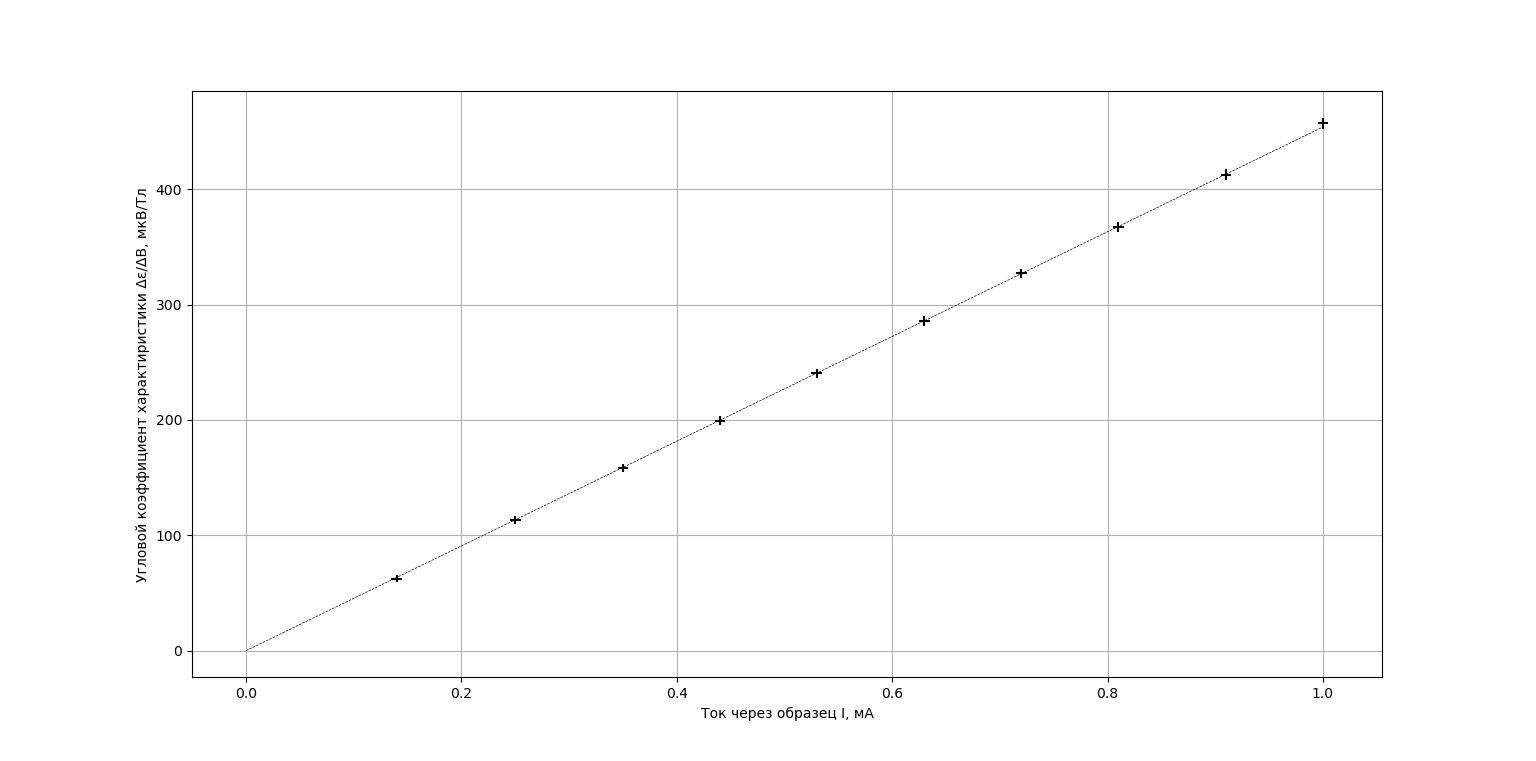
\includegraphics[scale = 0.33]{hhhui}
	\caption{Зависимость углового коэффициента $K$ характеристики от тока $I$ через образец. Прямая проведена с помощью МНК} \label{hhhui}
\end{figure} 

Теперь можем рассчитать концентрацию носителей тока в образце по формуле\[n=\frac{1}{eR_{\text{Х}}}=\left(2,35\pm0,03\right)\cdot10^{19}~\text{м}^{-3}=\left(2,35\pm0,03\right)\cdot10^{13}~\text{см}^{-3},\]что в пределах погрешности совпадает с табличным значением $n=2,33\cdot10^{13}~\text{см}^{-3}$.

\subsection*{III. Определение характера проводимости}

Определим знак носителей заряда. Это можно сделать, зная направление тока через образец, направление магнитного поля и знак ЭДС Холла. Направление тока в образце показано знаками $+$ и $-$ на его держателе. Направление тока в обмотках электромагнита покзано стрелкой не его торце. Отсюда можно определить направление магнитного поля в зазоре электромагнита, затем по правилу векторного произведения определить номер клеммы, к которой движутся холловские частицы. В нашем случае это клемма 3.

Подадим на образец небольшой ток и сравним показания вольтметра без магнитного поля и с полем. Видим, что знак ЭДС Холла -- $+$. Отсюда следует, что направление движения холловских частиц противоположно направлению напряжённости, вызванной эффектом Холла.

Значит, знак носителей заряда $-$.

\subsection*{IV. Определение удельной проводимости}

Выключим источник питания и удалим держатель с образцом из зазора. Подключим к клеммам вольтметра потенциальные концы 3 и 5 и измерим падение напряжения при токе $I=\left(1,000\pm0,005\right)~\text{мА}$. Оно равно $U_{3,5}=\left(2,494\pm0,015\right)~\text{мВ}$. Тогда удельная проводимость $\sigma$ германия может быть найдена по формуле\[\sigma=\frac{IL_{35}}{U_{35}al}=\left(1,982\pm0,019\right)\cdot10^3~\frac{1}{\Omega\cdot\text{м}},\]что в пределах погрешности совпадает с табличным значением $\sigma=2,0~\cdot10^3~\frac{1}{\Omega\cdot\text{м}}$.

Зная концентрацию и проводимость германия, можно вычислить подвижность носителей тока по формуле\[b=\frac{\sigma}{en}=\left(3,86\pm0,05\right)\cdot10^3~\frac{\text{см}^2}{\text{В}\cdot\text{с}}.\]Это с хорошей точностью совпадает со справочным значением $b=3,9\cdot10^3~\frac{\text{см}^2}{\text{В}\cdot\text{с}}$.

\section*{Вывод}

В данной работе был исследован эффект Холла в германии и были измерены подвижность и концентрация носителей заряда в полупроводниках.

В первой части работы была проведена градуировка используемого в работе электромагнита с помощью милливеберметра.

Во второй части работы были проведены измерения ЭДС Холла при различных величинах магнитного поля и тока через образец. В результате обработки данных получены линейные зависимости, совпадающие с теоретическими. По ним определена концентрация носителей заряда в германии. Она равна $n=\left(2,35\pm0,03\right)\cdot10^{13}~\text{см}^{-3}$, что в пределах погрешности совпадает со справочным значением $n=2,33\cdot10^{13}~\text{см}^{-3}$.

В третьей части работы был определён характер проводимости. Знак носителей заряда в германии $-$.

В четвёртой части была найдена удельная проводимость германия. Она оказалась равна $\sigma=\left(1,982\pm0,019\right)\cdot10^3~\frac{1}{\Omega\cdot\text{м}}$, что в пределах погрешности совпадает со справочным значением $\sigma=2,0~\cdot10^3~\frac{1}{\Omega\cdot\text{м}}$. Также была вычислена проводимость носителей тока как $b=\left(3,86\pm0,05\right)\cdot10^3~\frac{\text{см}^2}{\text{В}\cdot\text{с}}$, что в пределах погрешности совпадает со справочным значением $b=3,9\cdot10^3~\frac{\text{см}^2}{\text{В}\cdot\text{с}}$.

Относительно небольшие погрешности полученных значений и совпадение их со справочными говорит о корректности проведения эксперимента, правильности метода и исправной работе оборудования.

\end{document}
